
\newcommand{\xfill}[2][1ex]{{%
  \dimen0=#2\advance\dimen0 by #1
  \leaders\hrule height \dimen0 depth -#1\hfill%
}}

% This information is used in titlepage, colophon, preface and
% hyperref setup (pdf metainfo), and other options.

%\def\thesistypeabbr{B.Eng.}
\def\thesistype    {Bachelor of Engineering}
%\def\thesistypeabbr{B.Sc.Eng.}
%\def\thesistype    {Bachelor of Science in Engineering}
\def\thesistypeabbr{Đồ án tốt nghiệp Khoa học máy tính}
% \def\thesistype    {Master of Science in Engineering}
%\def\thesistypeabbr{Ph.D.}
%\def\thesistype    {Doctor of Philosophy}

\def\thesisauthor  {Hồ Đức Hưng}
\def\thesistitle   {\textrm{\LaTeX} thesis template for the Ho Chi Minh City University of Technology}
\def\thesissubtitle{A \emph{nice} thesis template}
\def\thesislocation{Hồ Chí Minh}

\def\papersize     {b5paper} % Final papersize (b5paper/a4paper), recommended papersize for DTU Compute is b5paper
\def\showtrims     {false} % Print on larger paper than \papersize and show trim marks (true/false)?

\def\showtodos     {true}  % Show todos (true/false)?
\def\confidential  {false} % Confidential thesis (true/false)?

\def \university {
    
    \noindent \huge {\textbf{Trường Đại Học Bách Khoa - ĐHQG HCM}} \\ \linespread{0.65}
    \LARGE {Khoa khoa học và kỹ thuật máy tính} \\ \linespread{0.65}
    \textcolor{dtured}{\rule{0.21\textwidth}{6pt}} \\*[1cm]
}

\RequirePackage[l2tabu,orthodox]{nag}
\RequirePackage{iftex}

\newcommand{\papersizeswitch}[3]{\ifnum\strcmp{\papersize}{#1}=0#2\else#3\fi}
%Change here the paper format
\papersizeswitch{b5paper}{\def\classfontsize{10pt}}{\def\classfontsize{12pt}}
\documentclass[\classfontsize,\papersize,twoside,showtrims,extrafontsizes]{memoir}
\usepackage{xhfill}
%%%%%%%%%%%%%%%%%%%%%%%%%%%%  PAPER SETTINGS    %%%%%%%%%%%%%%%%%%%%%%%%%%%%%%%%%
\showtrimsoff
\papersizeswitch{b5paper}{
    % Stock and paper layout
    \pagebv
    \setlrmarginsandblock{26mm}{20mm}{*}
    \setulmarginsandblock{35mm}{30mm}{*}
    \setheadfoot{8mm}{10mm}
    \setlength{\headsep}{7mm}
    \setlength{\marginparwidth}{18mm}
    \setlength{\marginparsep}{2mm}
}{
    \papersizeswitch{a4paper}{
        \pageaiv
        \setlength{\trimtop}{0pt}
        \setlength{\trimedge}{\stockwidth}
        \addtolength{\trimedge}{-\paperwidth}
        \settypeblocksize{634pt}{448.13pt}{*}
        \setulmargins{4cm}{*}{*}
        \setlrmargins{*}{*}{0.66}
        \setmarginnotes{17pt}{51pt}{\onelineskip}
        \setheadfoot{\onelineskip}{2\onelineskip}
        \setheaderspaces{*}{2\onelineskip}{*}
    }{}
}

\ifnum\strcmp{\showtrims}{true}=0
    % For printing B5 on A4 with trimmarks
    \showtrimson
    \papersizeswitch{b5paper}{\stockaiv}{\stockaiii}
    \setlength{\trimtop}{\stockheight}
    \addtolength{\trimtop}{-\paperheight}
    \setlength{\trimtop}{0.5\trimtop}
    \setlength{\trimedge}{\stockwidth}
    \addtolength{\trimedge}{-\paperwidth}
    \setlength{\trimedge}{0.5\trimedge}
    

    \trimLmarks
    
    % put jobname in left top trim mark
    \renewcommand*{\tmarktl}{%
      \begin{picture}(0,0)
        \unitlength 1mm
        \thinlines
        \put(-2,0){\line(-1,0){18}}
        \put(0,2){\line(0,1){18}}
        \put(3,15){\normalfont\ttfamily\fontsize{8bp}{10bp}\selectfont\jobname\ \
          \today\ \ 
          \printtime\ \ 
          Page \thepage}
      \end{picture}}

    % Remove middle trim marks for cleaner layout
    \renewcommand*{\tmarktm}{}
    \renewcommand*{\tmarkml}{}
    \renewcommand*{\tmarkmr}{}
    \renewcommand*{\tmarkbm}{}
\fi

\checkandfixthelayout                 % Check if errors in paper format!
\sideparmargin{outer}                 % Put sidemargins in outer position (why the fuck is this option not default by the class?)
%%%%%%%%%%%%%%%%%%%%%%%%%%%%%%%%%%%%%%%%%%%%%%%%%%%%%%%%%%%%%%

% Shows boundaries overlaid on the actual pages. Comment it to don't see them! 
%\usepackage{showframe}


% Large environments
\usepackage{microtype}
\usepackage{mathtools}
\usepackage{listings}                 % Source code printer for LaTeX
\usepackage{tikz}

% Mathematics
\usepackage{amsmath,dsfont,amsfonts,braket}
\usepackage{physics}
\usepackage[shortlabels]{enumitem}

% Citation & Acronyms
\usepackage{cite}
\usepackage{acronym}
\usepackage[hang,flushmargin]{footmisc} % Remove footnote indentation

% Modify Parts, Chapters, Sections...
\usepackage{titlesec}
\usepackage{fancyhdr}

% Links
\usepackage[hyphens]{url}             % Allow hyphens in URL's
\usepackage[unicode=false,psdextra]{hyperref}                 % References package

% Graphics, PDF files and colors
\usepackage{pdfpages}
\usepackage{graphicx}                 % Including graphics and using colours
\usepackage{subcaption}     % To use the environment "subfigure"
\usepackage{xcolor,colortbl}        % Defined more color names
\usepackage{eso-pic}                  % Watermark and other bag
\usepackage{preamble/dtucolors}
\graphicspath{{graphics/}}


% Language & Date
\ifPDFTeX
  \usepackage[vietnamese,danish,english]{babel}
  \usepackage[utf8]{inputenc}
\else
  % \usepackage{polyglossia}    % multilingual typesetting and appropriate hyphenation
  % \setdefaultlanguage{vietnamese}
  % \setotherlanguage{english}
  \usepackage[utf8]{inputenc}
  \usepackage[vietnamese]{babel}
\fi

\let\ordinal\relax % Avoids a warning due to incompatibility between Memoir class and <datetime>
\usepackage[nodayofweek]{datetime}
\usepackage[super]{nth}
\newdateformat{mydate}{\nth{\THEDAY}{ }\monthname[\THEMONTH] \THEYEAR} % Personal date style

% Floating objets, captions and references
\usepackage{flafter}  % floats is positioned after or where it is defined! 
%\setfloatlocations{figure}{bhtp}   % Set floats for all figures
%\setfloatlocations{table}{bhtp}    % Set floats for all tables
%\setFloatBlockFor{section}         % Typeset floats before each section
\usepackage[noabbrev,nameinlink,capitalise]{cleveref} % Clever references. Options: "fig. !1!" --> "!Figure 1!"
\DeclareCaptionFont{dtu}{\normalsize\sffamily\selectfont} %\fontsize{10.5}{10.5}
\usepackage[labelfont={dtu,bf},labelsep=period]{caption}
\captionsetup{font=small}
\captionnamefont{\bfseries}
\subcaptionlabelfont{\bfseries}
\newsubfloat{figure}
\newsubfloat{table}
%\letcountercounter{figure}{table}         % Consecutive table and figure numbering
%\letcountercounter{lstlisting}{table}     % Consecutive table and listings numbering
% strip things from equation references, making them "(1)" instead of "Equation~1"
% from http://tex.stackexchange.com/questions/122174/how-to-strip-eq-from-cleveref
\crefformat{equation}{(#2#1#3)}
\crefrangeformat{equation}{(#3#1#4) to~(#5#2#6)}
\crefmultiformat{equation}{(#2#1#3)}%
{ and~(#2#1#3)}{, (#2#1#3)}{ and~(#2#1#3)}

% Table of contents (TOC)
\setcounter{tocdepth}{3}              % Depth of table of content
\setcounter{secnumdepth}{-1}           % Depth of section numbering
\setcounter{maxsecnumdepth}{3}        % Max depth of section numbering


% Partstyle
\titleformat{\part}[display]{\filcenter\chapnamefont\fontsize{42pt}{0pt}\selectfont\setlength{\parskip}{-1.5cm}}{\vspace{4cm}\color{dtugray}{\chapnamefont\fontsize{36pt}{0pt}\selectfont}
\partname\chapnamefont\color{dtured}\fontsize{40pt}{0pt}\selectfont\hspace{.3em}\thepart}{4ex}{}
\titlespacing{\part}{0pt}{0pt}{0pt}


% Chapterstyle
\makeatletter
\makechapterstyle{mychapterstyle}{
    \chapterstyle{default}
    \def\format{\normalfont\sffamily}
    \setlength\beforechapskip{0mm}
    \renewcommand*{\chapnamefont}{\format\HUGE}
    \renewcommand*{\chapnumfont}{\format\fontsize{54}{54}\selectfont}
    \renewcommand*{\chaptitlefont}{\format\fontsize{42}{42}\selectfont}
    \renewcommand*{\printchaptername}{\chapnamefont\MakeUppercase{\@chapapp}}
    \patchcommand{\printchaptername}{\begingroup\color{dtugray}}{\endgroup}
    \renewcommand*{\chapternamenum}{\space\space}
    \patchcommand{\printchapternum}{\begingroup\color{dtured}}{\endgroup}
    \renewcommand*{\printchapternonum}{%
        \vphantom{\printchaptername\chapternamenum\chapnumfont 1}
        \afterchapternum}
    \setlength\midchapskip{1ex}
    \renewcommand*{\printchaptertitle}[1]{\raggedleft \chaptitlefont ##1}
    \renewcommand*{\afterchaptertitle}{\vskip0.5\onelineskip \hrule \vskip1.3\onelineskip}
}
\makeatother
\chapterstyle{mychapterstyle}


% Appendix page style
\renewcommand*{\cftappendixname}{Appendix\space} % Adds the word "Appendix" in ToC

\let\appendixpagenameorig\appendixpagename
\renewcommand{\appendixpagename}{\vspace{-2cm}\normalfont\sffamily\format\fontsize{42pt}{0pt}\selectfont\appendixpagenameorig} % Change font for the "Appendices" page

\renewcommand\appendixtocname{\large Appendices} % Change font dimension and name for "Appendices" in ToC

%%%%%%%%%%%%%%%%%%%%%%% Defines the protocol environment %%%%%%%%%%%%%%%%%%%%%

\newcounter{protocol}
\newenvironment{protocol}[1]
   {\par\addvspace{\topsep}
   \noindent
   \tabularx{\linewidth}{@{}>{\columncolor{dtured!8}[0pt][\tabcolsep]} X @{}}
   %{@{}>{\columncolor{gray!15}[0pt][\tabcolsep]}l|>{\columncolor{blue!25}}l|X|X@{}}
   %{@{} X @{}}
    %\hline
    \rule{0pt}{2.5ex}
    \refstepcounter{protocol}\textbf{\cellcolor{dtured!25}\large\sffamily Protocol \theprotocol} \large\sffamily#1 \\
    %\hline
    }
 { \\
    %\hline
   \endtabularx
   \par\addvspace{\topsep}}
%%%%%%%%%%%%%%%%%%%%%%%%%%%%%%%%%%%%%%%%%%%%%%%%%%%%%%%%%%%%%%%%%%%%%%%%

% Header and footer
\def\hffont{\sffamily\small}
\makepagestyle{myruled}
\makeheadrule{myruled}{\textwidth}{\normalrulethickness}
\makeevenhead{myruled}{\hffont\thepage}{}{\hffont\leftmark}
\makeoddhead{myruled}{\hffont\rightmark}{}{\hffont\thepage}
\makeevenfoot{myruled}{}{}{}
\makeoddfoot{myruled}{}{}{}
%%%%%% Adds the word "Appendix" to appendices header %%%
\makepagestyle{appruled}
\makeheadrule{appruled}{\textwidth}{\normalrulethickness}
\makeevenhead{appruled}{\hffont\thepage}{}{\hffont\appendixname~\leftmark}
\makeoddhead{appruled}{\hffont\appendixname~\rightmark}{}{\hffont\thepage}
\makeevenfoot{appruled}{}{}{}
\makeoddfoot{appruled}{}{}{}
%%%%%%%%%%%%%%%%%%%%%%%%%%%%%%%%%%%%%%%%%%%%%%%%%%%%%%%%
\makepsmarks{myruled}{
    \nouppercaseheads
    \createmark{chapter}{both}{shownumber}{}{\space}
    \createmark{section}{right}{shownumber}{}{\space}
    \createplainmark{toc}{both}{\contentsname}
    \createplainmark{lof}{both}{\listfigurename}
    \createplainmark{lot}{both}{\listtablename}
    \createplainmark{bib}{both}{\bibname}
    \createplainmark{index}{both}{\indexname}
    \createplainmark{glossary}{both}{\glossaryname}
}
\pagestyle{myruled}
\copypagestyle{cleared}{myruled}      % When \cleardoublepage, use myruled instead of empty
\makeevenhead{cleared}{\hffont\thepage}{}{} % Remove leftmark on cleared pages
\makeevenfoot{plain}{}{}{}            % No page number on plain even pages (chapter begin)
\makeoddfoot{plain}{}{}{}             % No page number on plain odd pages (chapter begin)


% \*section, \*paragraph font styles
\setsecheadstyle              {\huge\sffamily\raggedright}
\setsubsecheadstyle           {\LARGE\sffamily\raggedright}
\setsubsubsecheadstyle        {\Large\sffamily\raggedright}
%\setparaheadstyle             {\normalsize\sffamily\itseries\raggedright}
%\setsubparaheadstyle          {\normalsize\sffamily\raggedright}


% Hypersetup
\hypersetup{
    %pdfauthor={\thesisauthor{}},
    %pdftitle={\thesistitle{}},
    pdfdisplaydoctitle,
    bookmarksnumbered=true,
    bookmarksopen,
    breaklinks,
    linktoc=all,
    plainpages=false,
    unicode=true,
    colorlinks=false,
    citebordercolor=dtured,           % color of links to bibliography
    filebordercolor=dtured,           % color of file links
    linkbordercolor=dtured,           % color of internal links (change box color with linkbordercolor)
    urlbordercolor=blue,               % color of external links
    hidelinks,                        % Do not show boxes or colored links.
}



% Bibliography appearance in Table of Contents
\makeatletter
\renewcommand{\@memb@bchap}{%
  \ifnobibintoc\else
    \phantomsection
    \addcontentsline{toc}{part}{\bibname}%
  \fi
  \chapter*{\bibname}%
  \bibmark
  \prebibhook
}
\let\oldtableofcontents\tableofcontents
\newcommand{\newtableofcontents}{
    \@ifstar{\oldtableofcontents*}{
        \phantomsection\addcontentsline{toc}{chapter}{\contentsname}\oldtableofcontents*}}
\let\tableofcontents\newtableofcontents
\makeatother


% Confidential
\newcommand{\confidentialbox}[1]{
    \put(0,0){\parbox[b][\paperheight]{\paperwidth}{
        \begin{vplace}
            \centering
            \scalebox{1.3}{
                \begin{tikzpicture}
                    \node[very thick,draw=red!#1,color=red!#1,
                          rounded corners=2pt,inner sep=8pt,rotate=-20]
                          {\sffamily \HUGE \MakeUppercase{Confidential}};
                \end{tikzpicture}
            }
        \end{vplace}
    }}
}


% Prefrontmatter
\newcommand{\prefrontmatter}{
    \pagenumbering{alph}
    \ifnum\strcmp{\confidential}{true}=0
        \AddToShipoutPictureBG{\confidentialbox{10}}   % 10% classified box in background on each page
        \AddToShipoutPictureFG*{\confidentialbox{100}} % 100% classified box in foreground on first page
    \fi
}


% % DTU frieze
% \newcommand{\frieze}{%
%     \AddToShipoutPicture*{
%         \put(0,0){
%             \parbox[b][\paperheight]{\paperwidth}{%
%                 \includegraphics[trim=130mm 0 0 0,width=0.9\textwidth]{DTU-frise-SH-15}
%                 \vspace*{2.5cm}
%             }
%         }
%     }
% }

% % This is a double sided book. If there is a last empty page lets use it for some fun e.g. the frieze.
% % NB: For a fully functional hack the \clearpage used in \include does some odd thinks with the sequence numbering. Thefore use \input instead of \include at the end of the book. If bibliography is used at last everything should be ok.
% \makeatletter
% % Adjust so gatherings is allowd for single sheets too! (hacking functions in memoir.dtx)
% \patchcmd{\leavespergathering}{\ifnum\@memcnta<\tw@}{\ifnum\@memcnta<\@ne}{
%     \leavespergathering{1}
%     % Insert the frieze
%     \patchcmd{\@memensuresigpages}{\repeat}{\repeat\frieze}{}{}
% }{}
% \makeatother


%% Sharelatex fix for microtype warnings
\makeatletter
\def\MT@is@composite#1#2\relax{%
  \ifx\\#2\\\else
    \expandafter\def\expandafter\MT@char\expandafter{\csname\expandafter
                    \string\csname\MT@encoding\endcsname
                    \MT@detokenize@n{#1}-\MT@detokenize@n{#2}\endcsname}%
    % 3 lines added:
    \ifx\UnicodeEncodingName\@undefined\else
      \expandafter\expandafter\expandafter\MT@is@uni@comp\MT@char\iffontchar\else\fi\relax
    \fi
    \expandafter\expandafter\expandafter\MT@is@letter\MT@char\relax\relax
    \ifnum\MT@char@ < \z@
      \ifMT@xunicode
        \edef\MT@char{\MT@exp@two@c\MT@strip@prefix\meaning\MT@char>\relax}%
          \expandafter\MT@exp@two@c\expandafter\MT@is@charx\expandafter
            \MT@char\MT@charxstring\relax\relax\relax\relax\relax
      \fi
    \fi
  \fi
}
% new:
\def\MT@is@uni@comp#1\iffontchar#2\else#3\fi\relax{%
  \ifx\\#2\\\else\edef\MT@char{\iffontchar#2\fi}\fi
}
\makeatother




\usepackage{fontspec}

% Sans-serif font
\setsansfont[
    Ligatures=TeX,
    Extension=.otf,
    UprightFont=*-regular,
    BoldFont=*-bold,
    ItalicFont=*-italic,
    BoldItalicFont=*-bolditalic,
    %SlantedFont=,
    %BoldSlantedFont=,
    %SmallCapsFont=
    Scale=0.8      % Adjustmens when using math in sections
]{texgyreadventor}


%!TEX root = ../Thesis.tex

% Content specific packages.
\usepackage{blindtext}
\usepackage{listings}

% Listings
\colorlet{mygray}{black!30}
\colorlet{mygreen}{green!60!blue}
\colorlet{mymauve}{red!60!blue}

\lstset{
  % backgroundcolor=\color{gray!10},
  backgroundcolor=\color{white},
  basicstyle=\ttfamily,
  columns=fullflexible,
  breakatwhitespace=false,      
  breaklines=true,                
  captionpos=b,                    
  commentstyle=\color{mygreen}, 
  extendedchars=true,              
  frame=single,                   
  keepspaces=true,             
  keywordstyle=\color{blue},      
  language=python,                 
  numbers=left, %none                
  numbersep=5pt,                   
  numberstyle=\ttfamily\tiny\color{blue}, 
  rulecolor=\color{white},        
  showspaces=false,               
  showtabs=false,                 
  stepnumber=1,                  
  stringstyle=\color{mymauve},    
  tabsize=3,                      
  title=\lstname                
}



\begin{document}
\prefrontmatter
%!TEX root = ../Thesis.tex 
\thispagestyle{empty}             % No page numbers
\calccentering{\unitlength}
\begin{adjustwidth*}{\unitlength}{-\unitlength}
    \begin{adjustwidth}{-0.5cm}{-0.5cm}
        \sffamily
        \begin{flushright}
            \thesistype\\*[0cm]
            \thesistypeabbr \\
        \end{flushright}
        \vspace*{\fill}
        \noindent
        % 
\includegraphics[width=0.8\textwidth]{graphics/HCMUT.png}\\*[0.2cm]
        \university
        \HUGE \textbf{\thesistitle}\\*[0.6cm]
        % \huge \thesissubtitle \\*[0.6cm]
        \parbox[b]{0.5\linewidth}{
        \huge \thesisauthor\\*[1.2cm]
        \large\thesislocation{}, \the\year
        } 
        
        \hfill
\includegraphics[scale=0.14]{graphics/bklogo.png}
    \end{adjustwidth}
\end{adjustwidth*}
\normalfont
\normalsize

\cleartoevenpage
%!TEX root = ../Thesis.tex
\thispagestyle{empty} % No page numbers
% \frieze
\noindent
\sffamily

\large
\vspace*{\fill}
\hspace{-0.52cm}\textbf{Giáo viên hướng dẫn:} Prof. Sergio Leone\\
\textbf{Đồng hướng dẫn:} Prof. John Wayne \& Ass. Prof. Clint Eastwood
\vspace{5cm}

\small
% Leave the following empty spaces to avoid the Warning: "Underfull \hbox (badness 10000)"
\hspace*{\fill}\textbf{Đại Học Quốc Gia Hồ Chí Minh}

\hspace*{\fill}\textbf{Trường Đại Học Bách Khoa}

\hspace*{\fill}\textbf{Khoa Khoa Học Và Kỹ Thuật Máy Tính}

\hspace*{\fill}Cơ sở 1 (Đại học Bách Khoa)

\hspace*{\fill}Tòa nhà A3, 268 Lý Thường Kiệt, P.14, Quận 10

\hspace*{\fill} Thành Phố Hồ Chí Minh, Việt Nam


\normalsize
\normalfont
\vspace*{2cm}

\clearforchapter

\frontmatter
%!TEX root = ../Thesis.tex
\chapter{Summary}
\blindtext[2]


%!TEX root = ../Thesis.tex

\chapter{Preface}
\blindtext[2]

\vfill

{
\centering
    Kongens Lyngby, \mydate\today\\[.5cm]
    
\includegraphics[scale=0.2]{graphics/Signature.pdf}\\[.5cm]
\begin{center}
    Ross Moss
\end{center}
}
%!TEX root = ../Thesis.tex
\chapter{Acknowledgements}
\blindtext[2]

\chapter{List of publications}
Hopefully some.

\begin{itemize}
    \item First one
    \item Second one
    \item Maybe others
\end{itemize}
\chapter{Abbreviations}

\begin{acronym}[AVLAFTTT] % The name in the option ([...]) indicates the longest acronym to which the rest must align
\acro{AC}{Alternating current}
\acro{BS}{Beam-splitter}
\acro{DC}{Direct current}
\acro{AVLAFTTT}{A very long acronym for testing the option}
\end{acronym}
\clearforchapter
\phantomsection % This is added to make hyperref point to the right "Contents" page
\addcontentsline{toc}{part}{Mục lục} % Adds "Contents" as part-style in ToC
\tableofcontents*
\clearforchapter
\mainmatter
%!TEX root = ../Thesis.tex

\chapter*{Introduction}
\addcontentsline{toc}{part}{Introduction} % Adds "Introduction" as part-style in ToC
\markboth{Introduction}{Introduction}    % Marks left and right headers as "Introduction"

\begin{itemize}
    \item \textup{Upright shape}
    \item \textit{Italic shape}
    \item \textsl{Slanted shape}
    \item \textsc{Small Caps shape}
    \item \textmd{Medium series}
    \item \textbf{Bold sereies}
    \item \textrm{Roman family}
    \item \textsf{Sans serif family}
    \item \texttt{Typewriter family}
\end{itemize}

I love to write special characters like øæå indside my \TeX{} document. Also á, à, ü, û, ë, ê, î, ï could be nice. So waht about the ``π'' chracter. What about ° é ® † ¥ ü | œ π ‘ @ ö ä ¬ ∆ ‹ « © ƒ ∂ ß ª Ω … ç √ ∫ ñ µ ‚ · ¡ “ £ ∞ ™ [ ] ≠ ± '.

Some dashes - – —, and the latex form - -- ---
\begin{equation*}
    x = \mathtt{x}, \mathbf{x}, \mathit{x}, x_{1_{2_{3_{4}}}}^{1^{2^{3^{4}}}} \cdot hello * \text{hello world} ⋅ \text{my world} · \text{third world} ⊗ t
\end{equation*}

Lorem ipsum dolor sit amet, consectetur adipisicing elit, sed do eiusmod tempor incididunt ut labore et dolore magna aliqua. Ut enim ad minim veniam, quis nostrud exercitation ullamco laboris nisi ut aliquip ex ea commodo consequat. Duis aute irure dolor in reprehenderit in voluptate velit esse cillum dolore eu fugiat nulla pariatur. Excepteur sint occaecat cupidatat non proident, sunt in culpa qui officia deserunt mollit anim id est laborum \cite{adams1980hitchhiker}.

Mauris id quam non magna fermentum malesuada id mattis lorem. In a dapibus neque. Etiam lacus dui, malesuada ac eleifend imperdiet, imperdiet ut ipsum. Vestibulum id ultricies est. Phasellus augue mauris, semper a luctus vel, faucibus in risus. Fusce commodo augue quis elit sagittis non viverra turpis bibendum. Nunc placerat sem non sapien malesuada malesuada ullamcorper orci luctus \cite{adams1980hitchhiker}. Morbi pharetra ligula integer mollis mi nec neque ultrices vitae volutpat leo ullamcorper. In at tellus magna. Curabitur quis posuere purus. Cum sociis natoque penatibus et magnis dis parturient montes, nascetur ridiculus mus. Suspendisse tristique placerat feugiat. Aliquam vitae est at enim auctor ultrices eleifend a urna. Donec non tincidunt felis. Maecenas at suscipit orci. See \cref{myFigure}.

\begin{figure}
    \centering
    \caption[Short caption to special figure]{This is my special figure. Aliquam ultricies, arcu quis tempor rhoncus, tellus nisl tempus justo, condimentum tempor erat odio ac purus. Integer quis ipsum felis. Aliquam volutpat, leo ac consequat egestas, lectus lacus adipiscing quam, id iaculis dolor quam in erat. Phasellus tempor interdum arcu quis vestibulum}
    \label{myFigure}
\end{figure}

Fusce id suscipit sem. Aliquam venenatis nibh nec nisl luctus vel consectetur neque dapibus. Nulla feugiat egestas turpis, ac viverra eros cursus sit amet. Cras tincidunt felis vel tellus ultrices condimentum. Quisque vehicula, arcu vitae interdum dignissim, purus tortor cursus libero, sit amet accumsan quam magna in neque. Phasellus luctus leo odio. Aliquam ultricies, arcu quis tempor rhoncus, tellus nisl tempus justo, condimentum tempor erat odio ac purus. Integer quis ipsum felis. Aliquam volutpat, leo ac consequat egestas, lectus lacus adipiscing quam, id iaculis dolor quam in erat. Phasellus tempor interdum arcu quis vestibulum. Pellentesque sit amet augue purus. See \cref{myTable}.

\begin{table}
    \centering
        \begin{tabular}{c | r l}
            h & h & h \\
            e & e & e \\
        \end{tabular}
    \caption{This is a caption to the table}
    \label{myTable}
\end{table}
\newpage
\begin{lstlisting}
import numpy as np
    
def incmatrix(genl1,genl2):
    m = len(genl1)
    n = len(genl2)
    M = None #to become the incidence matrix
    VT = np.zeros((n*m,1), int)  #dummy variable
    
    #compute the bitwise xor matrix
    M1 = bitxormatrix(genl1)
    M2 = np.triu(bitxormatrix(genl2),1) 

    for i in range(m-1):
        for j in range(i+1, m):
            [r,c] = np.where(M2 == M1[i,j])
            for k in range(len(r)):
                VT[(i)*n + r[k]] = 1;
                VT[(i)*n + c[k]] = 1;
                VT[(j)*n + r[k]] = 1;
                VT[(j)*n + c[k]] = 1;
                
                if M is None:
                    M = np.copy(VT)
                else:
                    M = np.concatenate((M, VT), 1)
                
                VT = np.zeros((n*m,1), int)
    
    return M
\end{lstlisting}

\begin{figure}
    \centering
    \caption[Short caption to special figure]{This is my special figure. Aliquam ultricies, arcu quis tempor rhoncus, tellus nisl tempus justo, condimentum tempor erat odio ac purus. Integer quis ipsum felis. Aliquam volutpat, leo ac consequat egestas, lectus lacus adipiscing quam, id iaculis dolor quam in erat. Phasellus tempor interdum arcu quis vestibulum}
    \label{myFigure}
\end{figure}
\part{Theoretical concepts}
%!TEX root = ../Thesis.tex
%\chapter{Long chapter title with $\pi$ $π$ or π}
%\chapter{Long chapter title with \texorpdfstring{$\pi$ $π$ or π}{π π or π}}
 
\chapter{Long chapter}

My favorite RFC is \cite{rfc2549}.\blindtext[1]\\
Sans serif testing:
\begin{itemize}
    \item \textsf{$\pi$}
    \item \textsf{$π$}
    \item \textsf{π}
    \item \textsf{\emph{italic}}
    \item \textsf{\textbf{\emph{bold italic}}}
    \item \textsf{\textbf{bold}}
    \item \textsf{\texttt{teletype}}
    \item $\mathsf{Math\ Sans\ Serif}$
    \item \textsf{Text Sans Serif}
\end{itemize}

\section{Heading test}
\blindtext[8]
\subsection{Test 2}
\blindtext[1]

\part{Experimental techniques and results}
%!TEX root = ../Thesis.tex
%\chapter{Long chapter title with $\pi$ $π$ or π}
%\chapter{Long chapter title with \texorpdfstring{$\pi$ $π$ or π}{π π or π}}
 
\chapter{Experimental bla bla}

My favorite RFC is \cite{rfc2549}. This is a beam-splitter, \ac{BS}, hyper-ref test.\\

\noindent\blindtext[5]
\begin{protocol}{A cake}
\rule{0pt}{3ex}\textit{Ingredients}. Those you like the most.\\
\\
\textit{Preparation}. Mix the ingredients at your best.\\
\\
\textit{Baking}. Check it by eye.\\
\\
\textit{Final result}. Should be good.
\end{protocol}

%!TEX root = ../Thesis.tex
\chapter*{Conclusion}
\addcontentsline{toc}{part}{Conclusion} % Adds "Conclusion" as part-style in ToC
\markboth{Conclusion}{Conclusion}    % Marks left and right headers as "Introduction"

\blindtext[10]


\appendixpage\appendix
\pagestyle{appruled} % Comment to remove the word "Appendix" from the header
%!TEX root = ../Thesis.tex

\chapter{Journal articles}
\blindtext[5]\\

In case you want to  print your (hopefully) published papers in your phd thesis, this is a way to do it:
            
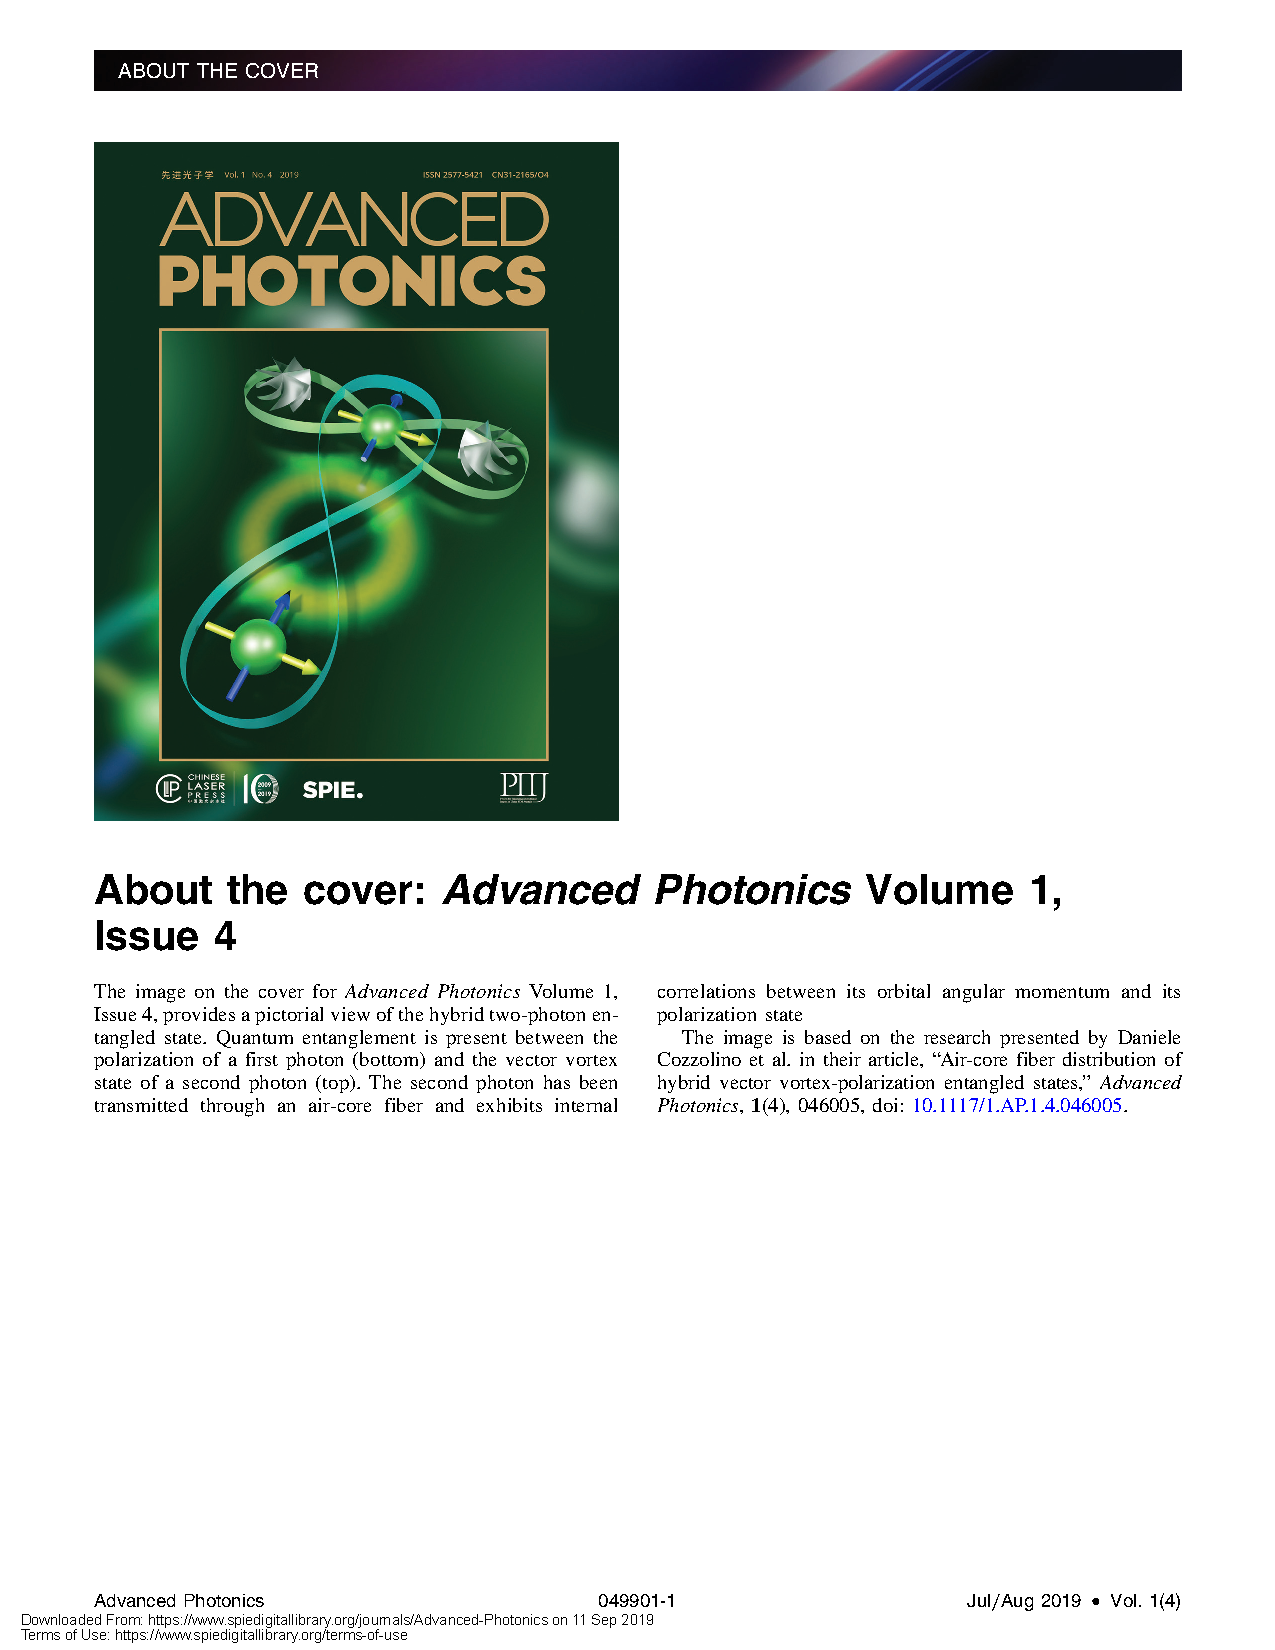
\includepdf[pages=-,
          pagecommand={\thispagestyle{empty}},
           scale=0.815,
           keepaspectratio]{appendices/Cover_AP.pdf} 


\backmatter
\pagestyle{myruled} %Restores the heading style as before "appruled". Remove if "appruled" is commented
\bibliography{bibliography/Bibliography.bib}
\bibliographystyle{ieeetr}
\end{document}


 

